\chapter{Intermolecular Forces and Solvents}\label{ch:b1:intermolecular-forces-solvents}

A gecko runs up a window pane and hangs from it by one toe; no glue, no
suction, only the attraction between the molecules of its toe pads and
those of the glass. Water, a molecule lighter than carbon dioxide, boils
at \qty{100}{\celsius}, while carbon dioxide is a gas at room
temperature. Oil floats on vinegar and never mixes with it; table
salt dissolves in water and not in petrol. All these facts are decided
not by the bonds inside molecules but by the much weaker forces between
them. This chapter classifies those forces, measures their effects on
boiling points, and uses them to choose a solvent.

% ledger: bp:H2O (the hook's 100 degC)

\begin{recall}
Book 1 (grade 11) introduced van der Waals forces and \omterm{def:b1:intermolecular-forces-solvents:hbond}{hydrogen bonds},
and explained that ionic solids dissolve by dissociation and \omterm{def:b1:intermolecular-forces-solvents:dissolution}{solvation}.
\omterm{def:b1:lewis-resonance-vsepr:dipole}{Dipole moments} were defined in \cref{def:b1:lewis-resonance-vsepr:dipole}
and \omterm{def:b1:periodicity:polarisability}{polarisability} in \cref{def:b1:periodicity:polarisability}. From
physics we use Coulomb's law: two charges $q_1$ and $q_2$ at a distance
$r$ in vacuum attract or repel with a force of norm $|q_1q_2|/(4\pi
\varepsilon_0 r^2)$.
\end{recall}

\begin{omfigure}
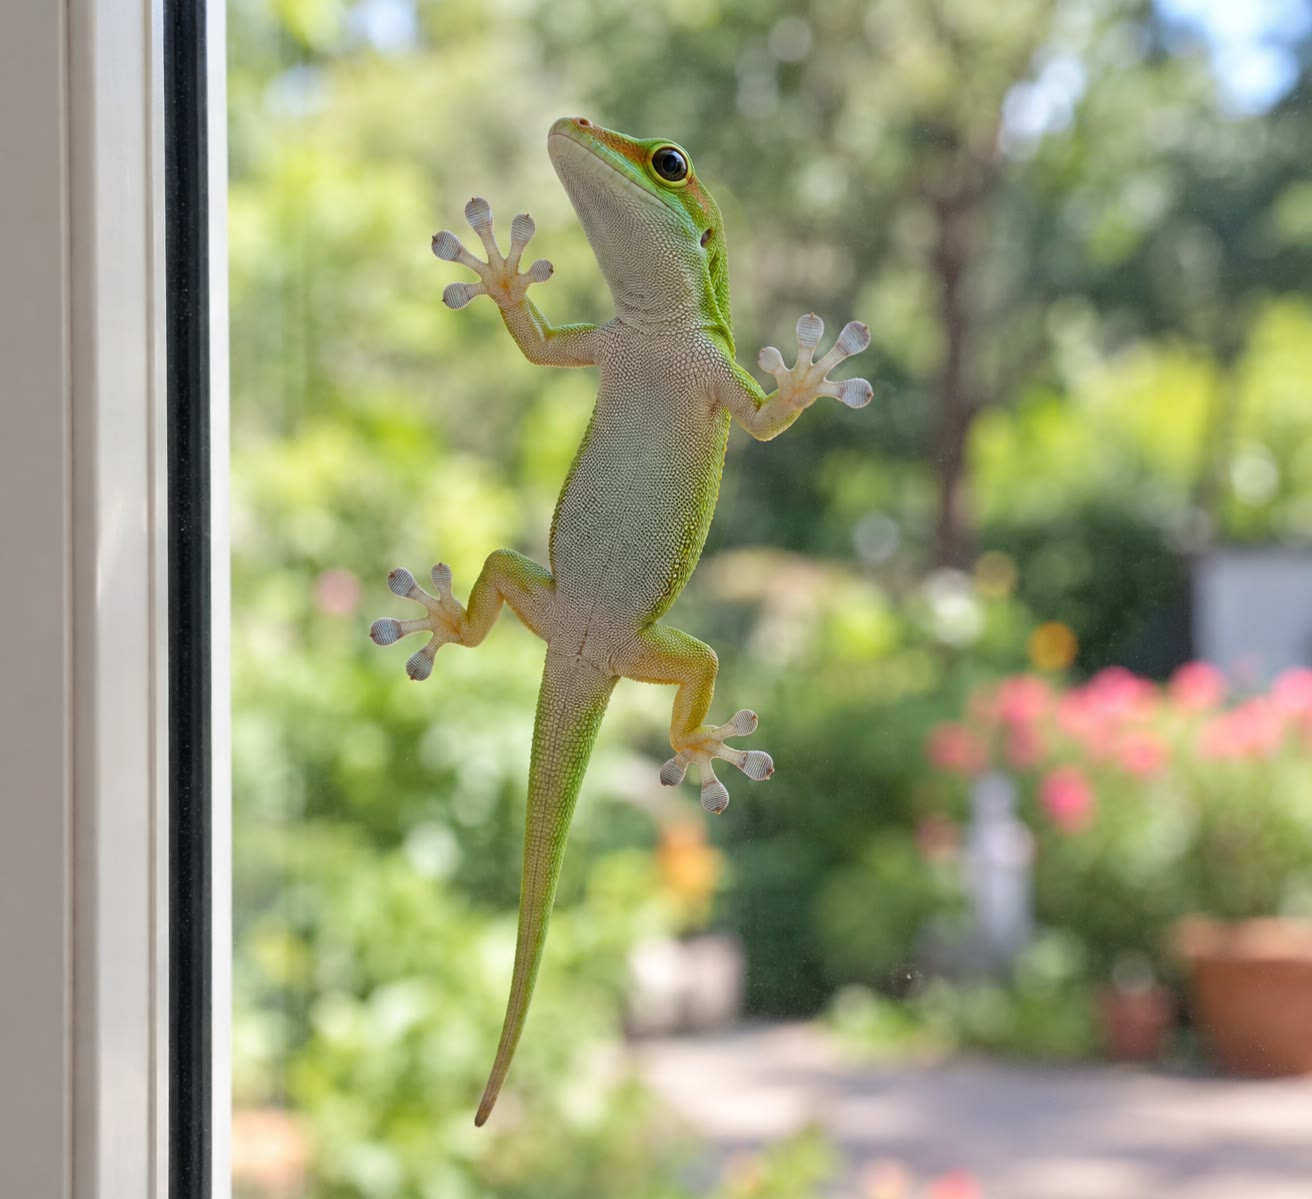
\includegraphics[width=0.52\linewidth]{images/book2/ai/b1-04-gecko.jpg}

{\small A gecko on a window pane. The millions of fine hairs of its toe
pads come so close to the glass that the weak attraction between their
molecules and those of the glass adds up to more than its weight.}
\end{omfigure}

\section{Van der Waals interactions}

\begin{definition}[Van der Waals interactions]\label{def:b1:intermolecular-forces-solvents:vdw}
The \emph{van der Waals interactions}\index{van der Waals interaction}
are the attractions between neutral molecules that come from the
interaction of their dipoles. Three kinds are distinguished:
\begin{itemize}
  \item the \emph{Keesom interaction}\index{Keesom interaction} (or
        orientation interaction) between two permanent dipoles, which
        tend to align head to tail;
  \item the \emph{Debye interaction}\index{Debye interaction} (or
        induction interaction) between a permanent dipole and the dipole
        it induces in a polarisable neighbour;
  \item the \emph{London interaction}\index{London interaction} (or
        dispersion interaction) between the instantaneous dipoles that the
        fluctuations of the electron clouds create in any two atoms or
        molecules, polar or not, and that induce each other.
\end{itemize}
\end{definition}

\begin{omfigure}
\begin{tikzpicture}[font=\small, >={Stealth},
    mol/.style={draw=black!60, fill=#1, ellipse, minimum width=1.5cm, minimum height=0.8cm}]
  % Keesom
  \node[mol=omDef!20] (a) at (0,0) {}; \node[mol=omDef!20] (b) at (1.7,0) {};
  \node at (-0.45,0) {$\delta^-$}; \node at (0.45,0) {$\delta^+$};
  \node at (1.25,0) {$\delta^-$}; \node at (2.15,0) {$\delta^+$};
  \node[below, align=center] at (0.85,-0.65) {Keesom:\\two permanent dipoles};
  % Debye
  \begin{scope}[xshift=4.6cm]
    \node[mol=omDef!20] at (0,0) {}; \node[mol=black!5, dashed] at (1.7,0) {};
    \node at (-0.45,0) {$\delta^-$}; \node at (0.45,0) {$\delta^+$};
    \node[omProp] at (1.25,0) {$\delta^-$}; \node[omProp] at (2.15,0) {$\delta^+$};
    \node[below, align=center] at (0.85,-0.65) {Debye:\\permanent and induced};
  \end{scope}
  % London
  \begin{scope}[xshift=9.2cm]
    \node[mol=black!5, dashed] at (0,0) {}; \node[mol=black!5, dashed] at (1.7,0) {};
    \node[omProp] at (-0.45,0) {$\delta^-$}; \node[omProp] at (0.45,0) {$\delta^+$};
    \node[omProp] at (1.25,0) {$\delta^-$}; \node[omProp] at (2.15,0) {$\delta^+$};
    \node[below, align=center] at (0.85,-0.65) {London:\\two instantaneous dipoles};
  \end{scope}
\end{tikzpicture}

{\small The three \omterm{def:b1:intermolecular-forces-solvents:vdw}{van der Waals interactions}. Black partial charges are
permanent (\omterm{def:b1:lewis-resonance-vsepr:dipole}{polar molecules}); orange ones are induced or instantaneous.
In each case the facing charges are opposite, so the molecules
attract.}
\end{omfigure}

\begin{proposition}[Strength and range]\label{prop:b1:intermolecular-forces-solvents:distance-law}
For two molecules at a distance $r$, each of the three van der Waals
energies varies as $-1/r^6$: the attraction is felt only between
neighbours. Their energies are of the order of a few kilojoules per
mole, about a hundred times less than a \omterm{def:b1:lewis-resonance-vsepr:lewis}{covalent bond}. The London term
grows with the polarisabilities of the two partners; it is present
between all molecules and is usually the largest of the three, except
for small very \omterm{def:b1:lewis-resonance-vsepr:dipole}{polar molecules}.
\end{proposition}
\admitted

\begin{example}[Noble gases and halogens]\label{ex:b1:intermolecular-forces-solvents:noble}
The atoms of a noble gas attract one another only by London forces,
which grow with the number of electrons: helium boils at
\qty{-268.9}{\celsius}, neon at \qty{-246.1}{\celsius}, argon at
\qty{-185.9}{\celsius}, krypton at \qty{-153.4}{\celsius}, xenon at
\qty{-108.1}{\celsius}. Likewise, at room temperature, difluorine and
dichlorine are gases, dibromine a liquid (boiling at \qty{58.8}{\celsius})
and diiodine a solid.
% ledger: bp:He, bp:Ne, bp:Ar, bp:Kr, bp:Xe, bp:F2, bp:Cl2, bp:Br2, bp:I2
\end{example}

\begin{omfigure}
\begin{tikzpicture}
\begin{axis}[
  width=0.62\linewidth, height=5.4cm,
  xmin=0.5, xmax=10.5, ymin=-180, ymax=200,
  axis x line=bottom, axis y line=left,
  xlabel={number of carbon atoms $n$}, ylabel={boiling point (\unit{\celsius})},
  xtick={1,2,3,4,5,6,7,8,9,10}, ytick={-150,-100,-50,0,50,100,150},
  tick label style={font=\small}, label style={font=\small}]
\addplot[omDef, thick, mark=*, mark size=1.5pt] table[x=n, y=bp_C] {figdata/out/bachelor-1-hydride-boiling-points-alkanes.dat};
\end{axis}
\end{tikzpicture}

{\small Boiling points of the linear alkanes \ce{C_nH_{2n+2}}, methane to
decane. Each added \ce{CH2} adds electrons and contact surface, hence
London attraction; the increment shrinks slowly, from about
\qty{75}{\celsius} at the start to \qty{25}{\celsius} at decane.}
\end{omfigure}

\section{The hydrogen bond}

\begin{definition}[Hydrogen bond]\label{def:b1:intermolecular-forces-solvents:hbond}
A \emph{hydrogen bond}\index{hydrogen bond} is an attraction
$\ce{X-H}\cdots\ce{Y}$ between a hydrogen atom bonded to a small, very
electronegative atom X (\ce{N}, \ce{O} or \ce{F}) and a \omterm{def:b1:lewis-resonance-vsepr:lewis}{lone pair} of
another electronegative atom Y. The molecule that carries \ce{X-H} is the
hydrogen-bond donor, the one that carries Y the acceptor. Its energy, 10
to \qty{40}{kJ/mol}, lies between \omterm{def:b1:intermolecular-forces-solvents:vdw}{van der Waals interactions} and \omterm{def:b1:lewis-resonance-vsepr:lewis}{covalent
bonds}; the three atoms \ce{X}, \ce{H}, \ce{Y} are nearly aligned.
\end{definition}

\begin{remark}[Why N, O and F]\label{rem:b1:intermolecular-forces-solvents:why}
A strongly electronegative X leaves hydrogen with a large partial
positive charge; hydrogen, which has no inner electrons, is tiny, so the
\omterm{def:b1:lewis-resonance-vsepr:lewis}{lone pair} of Y can come very close to it. Both conditions are needed:
\ce{C-H} bonds are not polar enough, and \ce{S-H} or \ce{Cl-H} bonds
involve atoms too large and too weakly electronegative to make strong
\omterm{def:b1:intermolecular-forces-solvents:hbond}{hydrogen bonds}.
\end{remark}

\begin{omfigure}
\begin{tikzpicture}[font=\small]
  % water network
  \foreach \n/\x/\y/\a in {1/0/0/0, 2/2.2/0.9/200, 3/0.2/-2.0/60, 4/-2.1/0.6/-30} {
    \begin{scope}[shift={(\x,\y)}, rotate=\a]
      \node[aO] (o\n) at (0,0) {};
      \node[aH] (h\n a) at (0.78,0.3) {};
      \node[aH] (h\n b) at (-0.2,-0.82) {};
      \begin{scope}[on background layer]
        \draw[bond] (o\n.center) -- (h\n a.center); \draw[bond] (o\n.center) -- (h\n b.center);
      \end{scope}
    \end{scope}
  }
  \draw[omThm, thick, densely dotted] (h1a) -- (o2);
  \draw[omThm, thick, densely dotted] (h1b) -- (o3);
  \draw[omThm, thick, densely dotted] (h4a) -- (o1);
  \node[below] at (0,-2.9) {water: each molecule can give two and accept two};
  % carboxylic acid dimer
  \begin{scope}[xshift=5.6cm, yshift=-0.6cm]
    \node (r1) at (-0.9,0) {R}; \node (c1) at (0,0) {C};
    \node (o1) at (0.6,0.85) {O}; \node (o2) at (0.6,-0.85) {O}; \node (h2) at (1.45,-0.85) {H};
    \node (c2) at (3.3,0) {C}; \node (r2) at (4.2,0) {R};
    \node (o3) at (2.7,0.85) {O}; \node (o4) at (2.7,-0.85) {O}; \node (h3) at (1.85,0.85) {H};
    \draw (r1) -- (c1) -- (o2) -- (h2) (c2) -- (r2) (c2) -- (o3) -- (h3);
    \draw[double, double distance=1.6pt] (c1) -- (o1); \draw[double, double distance=1.6pt] (c2) -- (o4);
    \draw[omThm, thick, densely dotted] (h2) -- (o4) (h3) -- (o1);
    \node[below] at (1.65,-2.3) {a carboxylic acid dimer};
  \end{scope}
\end{tikzpicture}

{\small \omterm{def:b1:intermolecular-forces-solvents:hbond}{Hydrogen bonds} (red dotted). In liquid water each molecule takes
part in up to four of them; carboxylic acids pair up in cyclic dimers
held by two \omterm{def:b1:intermolecular-forces-solvents:hbond}{hydrogen bonds}.}
\end{omfigure}

\begin{proposition}[Hydrogen bonds raise boiling points]\label{prop:b1:intermolecular-forces-solvents:hbond-bp}
Among the hydrides of \omterm{def:b1:periodicity:table}{groups} 15, 16 and 17, the boiling point increases
from \omterm{def:b1:periodicity:table}{period} 3 to \omterm{def:b1:periodicity:table}{period} 5, following the \omterm{def:b1:intermolecular-forces-solvents:vdw}{London interaction}; the
period-2 hydrides \ce{NH3}, \ce{H2O} and \ce{HF}, which form \omterm{def:b1:intermolecular-forces-solvents:hbond}{hydrogen
bonds}, boil far above the extrapolation of that trend. The hydrides of
\omterm{def:b1:periodicity:table}{group} 14 (\ce{CH4}, \ce{SiH4}, \ce{GeH4}) form no \omterm{def:b1:intermolecular-forces-solvents:hbond}{hydrogen bonds} and
follow the trend.
\end{proposition}

\begin{omfigure}
\begin{tikzpicture}
\begin{axis}[
  width=0.82\linewidth, height=6.6cm,
  xmin=1.5, xmax=5.6, ymin=-180, ymax=120,
  axis x line=bottom, axis y line=left,
  xlabel={period}, ylabel={boiling point (\unit{\celsius})},
  xtick={2,3,4,5}, ytick={-150,-100,-50,0,50,100},
  tick label style={font=\small}, label style={font=\small},
  clip=false]
\addplot[black!60, thick, mark=square*, mark size=1.6pt] table[x=period, y=bp_C] {figdata/out/bachelor-1-hydride-boiling-points-g14.dat};
\addplot[omDef, thick, mark=*, mark size=1.6pt] table[x=period, y=bp_C] {figdata/out/bachelor-1-hydride-boiling-points-g15.dat};
\addplot[omThm, thick, mark=*, mark size=1.6pt] table[x=period, y=bp_C] {figdata/out/bachelor-1-hydride-boiling-points-g16.dat};
\addplot[omMeth, thick, mark=triangle*, mark size=2pt] table[x=period, y=bp_C] {figdata/out/bachelor-1-hydride-boiling-points-g17.dat};
\addplot[omThm, dashed] coordinates {(2,-79.3) (3,-60.3)};
\node[font=\small, anchor=west] at (axis cs:2.05,100) {\ce{H2O}};
\node[font=\small, anchor=west] at (axis cs:2.05,19.6) {\ce{HF}};
\node[font=\small, anchor=west] at (axis cs:2.05,-30) {\ce{NH3}};
\node[font=\small, anchor=east] at (axis cs:1.96,-162) {\ce{CH4}};
\node[font=\small, anchor=west] at (axis cs:4.05,-41.3) {\ce{H2Se}};
\node[font=\small, anchor=west] at (axis cs:5.05,-18.4) {\ce{SbH3}};
\node[font=\small, anchor=west] at (axis cs:5.05,-35.1) {\ce{HI}};
\node[font=\small, anchor=west] at (axis cs:4.05,-88.1) {\ce{GeH4}};
\node[font=\small, omThm, anchor=north west] at (axis cs:2.05,-85) {extrapolated};
\end{axis}
\end{tikzpicture}

{\small Boiling points of the hydrides of \omterm{def:b1:periodicity:table}{group} 14 (grey squares), 15
(blue), 16 (red) and 17 (green). Water would boil near
\qty{-79}{\celsius} if it followed its heavier analogues (dashed); its
\omterm{def:b1:intermolecular-forces-solvents:hbond}{hydrogen bonds} raise it by about \qty{180}{\celsius}.}
% ledger: bp:CH4, bp:SiH4, bp:GeH4, bp:NH3, bp:PH3, bp:AsH3, bp:SbH3,
% bp:H2O, bp:H2S, bp:H2Se, bp:HF, bp:HCl, bp:HBr, bp:HI
\end{omfigure}

\begin{example}[Ethanol and its isomer]\label{ex:b1:intermolecular-forces-solvents:isomers}
Ethanol, \ce{CH3CH2OH}, and methoxymethane, \ce{CH3OCH3}, have the same
formula \ce{C2H6O} and nearly the same \omterm{def:b1:intermolecular-forces-solvents:vdw}{London interactions}. Ethanol,
whose \ce{O-H} group is both donor and acceptor, boils at
\qty{78.4}{\celsius}; methoxymethane, which can only accept, boils at
\qty{-25.0}{\celsius}.
% ledger: bp:C2H5OH, bp:CH3OCH3
\end{example}

\section{Solvents}

\begin{definition}[Relative permittivity]\label{def:b1:intermolecular-forces-solvents:permittivity}
In a medium, the Coulomb force between two charges is divided by a number
$\varepsilon_r \ge 1$, the \emph{relative permittivity}\index{relative permittivity}
(or dielectric constant) of the medium:
\[
  F = \frac{|q_1 q_2|}{4\pi\varepsilon_0\varepsilon_r r^2} .
\]
It is large for liquids of \omterm{def:b1:lewis-resonance-vsepr:dipole}{polar molecules}, which orient around the
charges and screen them: \num{78.4} for water at \qty{25}{\celsius},
\num{1.89} for hexane at \qty{20}{\celsius}.
% ledger: epsr:H2O, epsr:C6H14
\end{definition}

\begin{definition}[Polar, protic and aprotic solvents]\label{def:b1:intermolecular-forces-solvents:solvent-classes}
A \emph{polar solvent}\index{polar solvent} is made of molecules with a
large \omterm{def:b1:lewis-resonance-vsepr:dipole}{dipole moment} and has a large \omterm{def:b1:intermolecular-forces-solvents:permittivity}{relative permittivity} (above about
15); an apolar solvent has a small one. A \emph{protic
solvent}\index{protic solvent} has molecules that carry hydrogen atoms
able to form \omterm{def:b1:intermolecular-forces-solvents:hbond}{hydrogen bonds} (\ce{O-H} or \ce{N-H}); an \emph{aprotic
solvent}\index{aprotic solvent} has none.
\end{definition}

\begin{center}
\small
\begin{tabular}{lccll}
\hline
solvent & $\varepsilon_r$ & $\mu$ (D) & polarity & proticity \\
\hline
water & 78.4 & 1.86 & polar & protic \\
methanol & 32.6 & 1.67 & polar & protic \\
ethanol & 24.3 & 1.52 & polar & protic \\
acetonitrile, \ce{CH3CN} & 37.5 & 3.92 & polar & aprotic \\
propanone (acetone) & 20.7 & 2.88 & polar & aprotic \\
dichloromethane & 9.08 & 1.62 & weakly polar & aprotic \\
ethyl ethanoate & 6.02 & 1.78 & weakly polar & aprotic \\
ethoxyethane & 4.34 & 1.15 & weakly polar & aprotic \\
benzene & 2.28 & 0 & apolar & aprotic \\
hexane & 1.89 & 0 & apolar & aprotic \\
\hline
\end{tabular}
\end{center}
% ledger: epsr:H2O, epsr:CH3OH, epsr:C2H5OH, epsr:CH3CN, epsr:CH3COCH3,
% epsr:CH2Cl2, epsr:EtOAc, epsr:Et2O, epsr:C6H6, epsr:C6H14, dip:H2O,
% dip:CH3OH, dip:C2H5OH, dip:CH3CN, dip:CH3COCH3, dip:CH2Cl2, dip:EtOAc,
% dip:Et2O, dip:C6H6 (relative permittivities at 20 or 25 degC; dipole
% moments of the gas-phase molecules; hexane has no dipole by symmetry)

\begin{definition}[Solvation, ionising and dissociating power]\label{def:b1:intermolecular-forces-solvents:dissolution}
The \emph{solvation}\index{solvation} of a solute particle is its
surrounding by solvent molecules oriented and bound to it by
intermolecular forces (hydration, in water). The \emph{ionising
power}\index{ionising power} of a solvent is its ability to turn a
polar \omterm{def:b1:lewis-resonance-vsepr:lewis}{covalent bond} of the solute into an ion pair, a property of
\omterm{def:b1:intermolecular-forces-solvents:solvent-classes}{polar solvents} with a large \omterm{def:b1:lewis-resonance-vsepr:dipole}{dipole moment}; its \emph{dissociating
power}\index{dissociating power} is its ability to separate the ions of
a pair, measured by its \omterm{def:b1:intermolecular-forces-solvents:permittivity}{relative permittivity}.
\end{definition}

\begin{proposition}[Dissolving in three steps]\label{prop:b1:intermolecular-forces-solvents:steps}
The dissolution of an electrolyte in a solvent can be described in three
steps: ionisation (for a molecular solute such as \ce{HCl}), dissociation
of the ion pairs, and \omterm{def:b1:intermolecular-forces-solvents:dissolution}{solvation} of the separated ions. A solvent dissolves
an ionic or very polar solute well when it is polar (ionising), of high
permittivity (dissociating) and able to solvate both ions --- the
cations by its \omterm{def:b1:lewis-resonance-vsepr:lewis}{lone pairs}, the anions by \omterm{def:b1:intermolecular-forces-solvents:hbond}{hydrogen bonds} if it is protic.
Water does all three.
\end{proposition}

\begin{example}[Hydrogen chloride in water and in hexane]\label{ex:b1:intermolecular-forces-solvents:hcl}
In water, \ce{HCl} is ionised and dissociated completely:
\ce{HCl(g) + H2O(l) -> H3O+(aq) + Cl-(aq)}; the solution conducts. In
hexane, apolar and of low permittivity, it dissolves as \ce{HCl}
molecules and the solution does not conduct.
\end{example}

\begin{omfigure}
\begin{tikzpicture}[font=\small]
  \node[aNa] (na) at (0,0) {};
  \node[font=\scriptsize, white] at (na) {\ce{Na+}};
  \foreach \a in {0,60,...,300} {
    \begin{scope}[shift={(\a:1.25)}, rotate=\a]
      \node[aO] (o) at (0,0) {};
      \node[aH] (ha) at (0.55,0.5) {}; \node[aH] (hb) at (0.55,-0.5) {};
      \begin{scope}[on background layer]
        \draw[bond] (o.center) -- (ha.center); \draw[bond] (o.center) -- (hb.center);
      \end{scope}
    \end{scope}
  }
  \node[below] at (0,-2.4) {cation: oxygen lone pairs inward};
  \begin{scope}[xshift=6.2cm]
    \node[aCl] (cl) at (0,0) {};
    \node[font=\scriptsize, white] at (cl) {\ce{Cl-}};
    \foreach \a in {0,60,...,300} {
      \begin{scope}[shift={(\a:1.55)}, rotate=\a]
        \node[aH] (h1) at (-0.62,0) {};
        \node[aO] (o) at (0,0) {};
        \node[aH] (h2) at (0.25,0.72) {};
        \begin{scope}[on background layer]
          \draw[bond] (o.center) -- (h1.center); \draw[bond] (o.center) -- (h2.center);
        \end{scope}
      \end{scope}
    }
    \node[below] at (0,-2.4) {anion: hydrogen bonds inward};
  \end{scope}
\end{tikzpicture}

{\small Hydration of the two ions of sodium chloride (first layer only,
drawn in the plane). Water turns its negative end, oxygen, towards the
cation, and one hydrogen towards the anion.}
\end{omfigure}

\section{Solubility, miscibility and amphiphiles}

\begin{proposition}[Like dissolves like]\label{prop:b1:intermolecular-forces-solvents:like}
A solute dissolves well in a solvent when the interactions between solute
and solvent molecules are comparable to those they lose: polar or
ion-forming solutes in \omterm{def:b1:intermolecular-forces-solvents:solvent-classes}{polar solvents}, apolar solutes in apolar
solvents, hydrogen-bonding solutes in \omterm{def:b1:intermolecular-forces-solvents:solvent-classes}{protic solvents}.
\end{proposition}

\begin{proof}[Reasoning]
Dissolving breaks solute--solute and solvent--solvent interactions and
makes solute--solvent ones. If the solute is apolar and the solvent water,
the water molecules lose \omterm{def:b1:intermolecular-forces-solvents:hbond}{hydrogen bonds} to make room for it and gain only
weak \omterm{def:b1:intermolecular-forces-solvents:vdw}{London interactions} in exchange: dissolution is unfavourable. If
both are apolar, the \omterm{def:b1:intermolecular-forces-solvents:vdw}{London interactions} lost and gained are comparable,
and mixing is favoured by the disorder it creates.
\end{proof}

\begin{definition}[Miscible liquids]\label{def:b1:intermolecular-forces-solvents:miscibility}
Two liquids are \emph{miscible}\index{miscible} when they mix in all
proportions into a single liquid phase; otherwise they form two layers,
the less dense on top.
\end{definition}

\begin{example}[Water with ethanol, water with hexane]\label{ex:b1:intermolecular-forces-solvents:miscible}
Ethanol is \omterm{def:b1:intermolecular-forces-solvents:miscibility}{miscible} with water: both are protic and polar, and ethanol
hydrogen-bonds with water as well as with itself. Hexane and water are
immiscible. Diiodine, a molecular solid, is barely soluble in water but
dissolves readily in hexane or dichloromethane: shaken with such a
solvent, aqueous iodine passes into the organic layer, the principle of
liquid--liquid extraction (\cref{ch:b1:lab-techniques-1}).
\end{example}

\begin{omfigure}
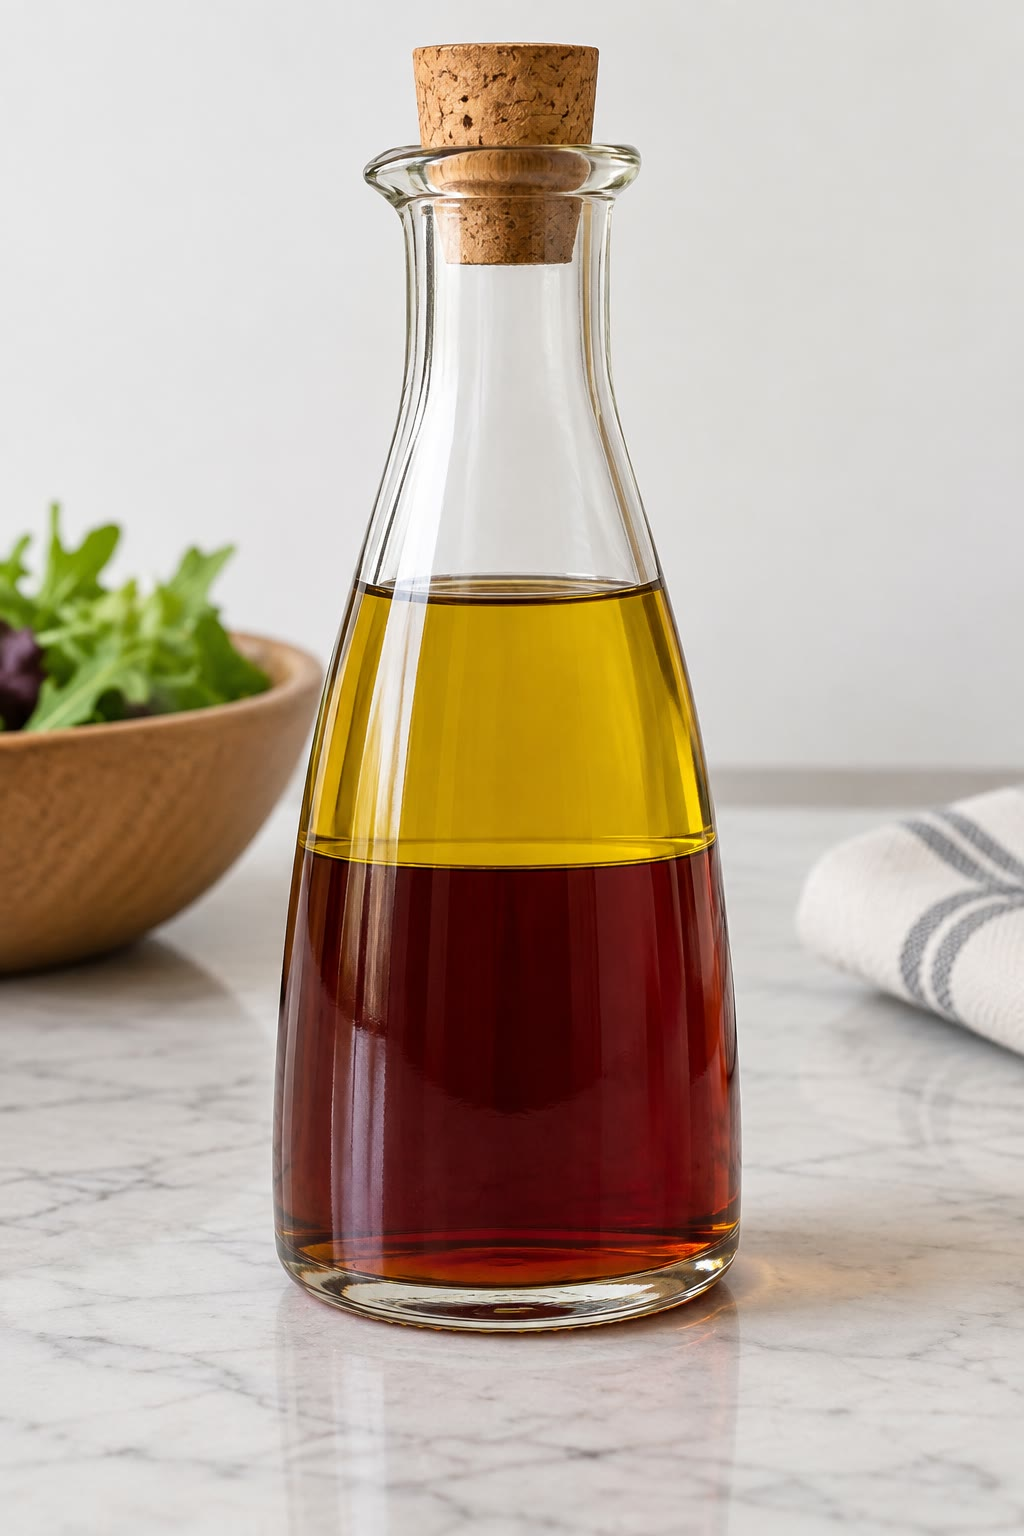
\includegraphics[width=0.2\linewidth]{images/book2/ai/b1-04-dressing.jpg}

{\small A salad dressing at rest: olive oil, apolar, floats on vinegar,
an aqueous solution; the two liquids are immiscible.}
\end{omfigure}

\begin{definition}[Hydrophilic, hydrophobic, amphiphilic]\label{def:b1:intermolecular-forces-solvents:amphiphile}
A group is \emph{hydrophilic}\index{hydrophilic} when it interacts
favourably with water (ionic or polar groups: \ce{-COO^-}, \ce{-OH},
\ce{-SO3^-}) and \emph{hydrophobic}\index{hydrophobic} when it does not
(hydrocarbon chains). A molecule is \emph{amphiphilic}\index{amphiphilic}
when it carries both a hydrophilic head and a hydrophobic tail.
\end{definition}

\begin{example}[Soap]\label{ex:b1:intermolecular-forces-solvents:soap}
Sodium dodecanoate, \ce{CH3(CH2)10COO- Na+}, is \omterm{def:b1:intermolecular-forces-solvents:amphiphile}{amphiphilic}. At the
surface of water its molecules stand with the head in the water and the
tail in the air. In the bulk, above a small concentration, they gather
into spheres --- micelles --- with the tails inside and the heads
outside. Grease, apolar, dissolves in the \omterm{def:b1:intermolecular-forces-solvents:amphiphile}{hydrophobic} core of the micelles
and is carried away by the water.
\end{example}

\begin{omfigure}
\begin{tikzpicture}[font=\small]
  % interface
  \fill[omWater] (-3.2,-1.6) rectangle (-0.4,0);
  \draw[omDef!60] (-3.2,0) -- (-0.4,0);
  \node[anchor=south west] at (-3.2,0.95) {air};
  \node[anchor=north west] at (-3.2,-1.2) {water};
  \foreach \x in {-2.9,-2.5,...,-0.6} {
    \fill[omThm] (\x,-0.12) circle (0.11);
    \draw[thick, black!70, decorate, decoration={zigzag, amplitude=1pt, segment length=3pt}] (\x,0) -- (\x,0.85);
  }
  % micelle
  \begin{scope}[xshift=3.2cm, yshift=-0.4cm]
    \fill[omWater] (-2,-1.6) rectangle (2,1.6);
    \foreach \a in {0,30,...,330} {
      \draw[thick, black!70, decorate, decoration={zigzag, amplitude=1pt, segment length=3pt}] (\a:0.25) -- (\a:1.0);
      \fill[omThm] (\a:1.12) circle (0.11);
    }
    \node[anchor=north] at (0,-1.65) {a micelle in water};
  \end{scope}
\end{tikzpicture}

{\small \omterm{def:b1:intermolecular-forces-solvents:amphiphile}{Amphiphilic} molecules (red \omterm{def:b1:intermolecular-forces-solvents:amphiphile}{hydrophilic} head, zigzag \omterm{def:b1:intermolecular-forces-solvents:amphiphile}{hydrophobic}
tail) at the surface of water and gathered into a micelle, drawn in
cross-section; micelles are studied in the Year 3 volume.}
\end{omfigure}

\begin{method}[Choosing a solvent]\label{met:b1:intermolecular-forces-solvents:choose}
To choose a solvent for a solute or a reaction:
\begin{enumerate}
  \item characterise the solute: ionic, polar, able to give or accept
        \omterm{def:b1:intermolecular-forces-solvents:hbond}{hydrogen bonds}, or apolar;
  \item choose a solvent of the same kind (\cref{prop:b1:intermolecular-forces-solvents:like}),
        with a high permittivity if ions must be separated;
  \item for a reaction between an anion and a molecule, prefer a polar
        \omterm{def:b1:intermolecular-forces-solvents:solvent-classes}{aprotic solvent}, which dissolves the salt without binding the
        anion by \omterm{def:b1:intermolecular-forces-solvents:hbond}{hydrogen bonds} (\cref{ch:b1:nucleophilic-substitution});
  \item for an extraction, choose a solvent immiscible with the first one
        and in which the solute is much more soluble.
\end{enumerate}
\end{method}

\section{Exercises}

\begin{exercise}[$\star$]\label{exo:b1:intermolecular-forces-solvents:1}
Name the interactions present between the particles of liquid argon,
liquid hydrogen chloride, liquid water, liquid methane and solid
diiodine, and say which dominates in each.
\end{exercise}

\begin{exercise}[$\star$]\label{exo:b1:intermolecular-forces-solvents:2}
Which of these substances form \omterm{def:b1:intermolecular-forces-solvents:hbond}{hydrogen bonds} between their own
molecules: \ce{CH3OH}, \ce{CH3OCH3}, \ce{CH3NH2}, \ce{CH3F}, \ce{HF},
\ce{CH4}? Which can only accept \omterm{def:b1:intermolecular-forces-solvents:hbond}{hydrogen bonds} from another molecule?
\end{exercise}

\begin{exercise}[$\star$]\label{exo:b1:intermolecular-forces-solvents:3}
Using the table of solvents, classify water, ethanol, propanone, hexane,
dichloromethane and acetonitrile as polar or apolar, protic or aprotic.
\end{exercise}

\begin{exercise}[$\star$]\label{exo:b1:intermolecular-forces-solvents:4}
Explain why diiodine dissolves much better in hexane than in water, and
why sodium chloride does the opposite.
\end{exercise}

\begin{exercise}[$\star\star$]\label{exo:b1:intermolecular-forces-solvents:5}
Methanol boils at \qty{64.7}{\celsius}, ethanol at \qty{78.4}{\celsius},
ethanoic acid at \qty{118.1}{\celsius} and methoxymethane at
\qty{-25.0}{\celsius}. Explain the order.
% ledger: bp:CH3OH, bp:C2H5OH, bp:CH3COOH, bp:CH3OCH3
\end{exercise}

\begin{exercise}[$\star\star$]\label{exo:b1:intermolecular-forces-solvents:6}
Compute the Coulomb force between a \ce{Na+} and a \ce{Cl-} ion
\qty{500}{pm} apart in vacuum ($\varepsilon_0 = \qty{8.854e-12}{F/m}$,
$e = \qty{1.602e-19}{C}$), then in water ($\varepsilon_r = 78.4$) and in
hexane ($\varepsilon_r = 1.89$). Comment.
\end{exercise}

\begin{exercise}[$\star\star$]\label{exo:b1:intermolecular-forces-solvents:7}
Propanone and water are \omterm{def:b1:intermolecular-forces-solvents:miscibility}{miscible} in all proportions; hexane and water are
not. Explain, considering the interactions broken and formed.
\end{exercise}

\begin{exercise}[$\star\star$]\label{exo:b1:intermolecular-forces-solvents:8}
\ce{HCl} has a \omterm{def:b1:lewis-resonance-vsepr:dipole}{dipole moment} of \qty{1.09}{\debye} and boils at
\qty{-85.0}{\celsius}; \ce{HBr} has \qty{0.83}{\debye} and boils at
\qty{-66.4}{\celsius}. Why does the less \omterm{def:b1:lewis-resonance-vsepr:dipole}{polar molecule} boil higher?
% ledger: dip:HCl, dip:HBr, bp:HCl, bp:HBr
\end{exercise}

\begin{exercise}[$\star\star$]\label{exo:b1:intermolecular-forces-solvents:9}
Draw the cyclic dimer of ethanoic acid. In benzene solution, ethanoic
acid behaves as if its molar mass were about twice \qty{60}{g/mol}; in
water it does not. Explain both facts.
\end{exercise}

\begin{exercise}[$\star\star\star$]\label{exo:b1:intermolecular-forces-solvents:10}
Describe the dissolution of sodium chloride in water in terms of
dissociation and \omterm{def:b1:intermolecular-forces-solvents:dissolution}{solvation}, and that of hydrogen chloride in water in
terms of ionisation, dissociation and \omterm{def:b1:intermolecular-forces-solvents:dissolution}{solvation}. Why does hydrogen
chloride in hexane give a non-conducting solution?
\end{exercise}

\begin{exercise}[$\star\star\star$]\label{exo:b1:intermolecular-forces-solvents:11}
From the boiling points of the linear alkanes (pentane
\qty{36.1}{\celsius}, decane \qty{174.1}{\celsius}), compute the mean
increase per \ce{CH2} group between \ce{C5} and \ce{C10}, and estimate
the boiling point of undecane. Why does the increment decrease along the
series?
% ledger: bp:C5H12, bp:C10H22
\end{exercise}

\begin{exercise}[$\star\star\star$]\label{exo:b1:intermolecular-forces-solvents:12}
Sodium dodecyl sulfate, \ce{CH3(CH2)11OSO3^- Na+}, is a detergent. Identify
its \omterm{def:b1:intermolecular-forces-solvents:amphiphile}{hydrophilic} and \omterm{def:b1:intermolecular-forces-solvents:amphiphile}{hydrophobic} parts, sketch its arrangement at the
surface of water and in a micelle, and explain how it removes an oily
stain from a fabric.
\end{exercise}

\section{Problem: If Water Had No Hydrogen Bonds}

\begin{problem}[{Weekend problem --- London forces in the noble gases and
the alkanes, the choice of a solvent, and the boiling point water would
have without hydrogen bonds}]
\label{pb:b1:intermolecular-forces-solvents:1}
Boiling points under \qty{1}{atm} (in \unit{\celsius}): \ce{He} $-268.9$,
\ce{Ne} $-246.1$, \ce{Ar} $-185.9$, \ce{Kr} $-153.4$, \ce{Xe} $-108.1$;
pentane 36.1, hexane 68.8; \ce{CH4} $-161.5$, \ce{SiH4} $-112.0$,
\ce{GeH4} $-88.1$; \ce{NH3} $-33.4$, \ce{PH3} $-87.8$, \ce{AsH3} $-62.5$;
\ce{H2O} 100.0, \ce{H2S} $-60.3$, \ce{H2Se} $-41.3$; \ce{HF} 19.6,
\ce{HCl} $-85.0$, \ce{HBr} $-66.4$.
% ledger: bp:He, bp:Ne, bp:Ar, bp:Kr, bp:Xe, bp:C5H12, bp:C6H14, bp:CH4,
% bp:SiH4, bp:GeH4, bp:NH3, bp:PH3, bp:AsH3, bp:H2O, bp:H2S, bp:H2Se,
% bp:HF, bp:HCl, bp:HBr

\medskip
\noindent\textbf{Part I --- London alone.}
\begin{enumerate}
  \item Which interaction holds the atoms of liquid argon together?
  \item Explain the increase of the boiling point from helium to xenon.
  \item Why is the boiling point of helium the lowest of all substances?
  \item Compare pentane and hexane: what does one \ce{CH2} group add?
  \item Methane, silane and germane have no \omterm{def:b1:lewis-resonance-vsepr:dipole}{dipole moment}. Which
        interaction explains the order of their boiling points?
  \item Why is no \omterm{def:b1:intermolecular-forces-solvents:hbond}{hydrogen bond} possible in methane?
\end{enumerate}

\medskip
\noindent\textbf{Part II --- Choosing solvents.}
Use the table of solvents of the chapter.
\begin{enumerate}[resume]
  \item Which solvent of the table dissolves sodium chloride best, and
        why?
  \item By what factor is the attraction between two ions smaller in
        water than in hexane at the same distance?
  \item A reaction between the anion \ce{CN-} and an organic molecule
        should be run in a solvent that dissolves the salt but does not
        bind the anion by \omterm{def:b1:intermolecular-forces-solvents:hbond}{hydrogen bonds}. Choose one.
  \item To extract diiodine from an aqueous solution, which solvent of the
        table would you choose, and in which layer will the iodine end?
  \item Explain why ethanol cannot be used for that extraction.
  \item Ethoxyethane is barely \omterm{def:b1:intermolecular-forces-solvents:miscibility}{miscible} with water although it is polar.
        Propose an explanation.
\end{enumerate}

\medskip
\noindent\textbf{Part III --- The other hydrides.}
\begin{enumerate}[resume]
  \item For \omterm{def:b1:periodicity:table}{group} 17, compute the change of boiling point from \ce{HCl} to
        \ce{HBr}, and extrapolate the same change back to \omterm{def:b1:periodicity:table}{period} 2.
  \item Compare the extrapolated value with the boiling point of \ce{HF}.
  \item Same two questions for \omterm{def:b1:periodicity:table}{group} 15 (\ce{PH3}, \ce{AsH3} and
        \ce{NH3}).
  \item For \omterm{def:b1:periodicity:table}{group} 14, does \ce{CH4} lie above or below the extrapolation
        from \ce{SiH4} and \ce{GeH4}? Why is that not surprising?
  \item Rank the excesses of \ce{NH3}, \ce{HF} and water.
  \item Count the \omterm{def:b1:intermolecular-forces-solvents:hbond}{hydrogen bonds} each molecule of \ce{NH3}, \ce{HF} and
        \ce{H2O} can give and accept, and explain the ranking.
\end{enumerate}

\medskip
\noindent\textbf{Part IV --- Water without \omterm{def:b1:intermolecular-forces-solvents:hbond}{hydrogen bonds}.}
\begin{enumerate}[resume]
  \item Why are \ce{H2S} and \ce{H2Se} suitable for an extrapolation, and
        why not water itself?
  \item Compute the change of boiling point from \ce{H2S} to \ce{H2Se}.
  \item Write the equation of the straight line through these two points,
        with the \omterm{def:b1:periodicity:table}{period} $p$ as variable.
  \item Deduce the boiling point water would have at $p = 2$.
  \item By how much do \omterm{def:b1:intermolecular-forces-solvents:hbond}{hydrogen bonds} raise the boiling point of water?
  \item Conclude: at what temperature would water boil if its molecules
        attracted one another like those of \ce{H2S}?
\end{enumerate}
\end{problem}
